\documentclass[12pt]{article}
\usepackage[utf8]{inputenc}
\usepackage[croatian]{babel}
\usepackage{tocloft}
\usepackage{titlesec}
\usepackage{float}
\usepackage{graphicx}
\usepackage{hyperref}

\setlength{\parindent}{4em}
\setlength{\parskip}{1em}
\renewcommand{\baselinestretch}{1.175}

\titlelabel{\thetitle.\quad}
\renewcommand{\cftsecleader}{\cftdotfill{\cftdotsep}}

\begin{document}

\title{\textbf{Multimedijski sustavi} \\
\large Završni projekt}
\author{\underline{Autor:} Lucija Valentić, 1191236528 }
\date{\underline{Naziv:} Super Kirlia}

\maketitle
\newpage

\font\myfont=cmr12 at 10pt

\tableofcontents
\newpage

\section{Uvod}
Za svoj završni projekt iz predmeta Multimedijski sustavi sam odlučila napraviti jednu jednostavnu igru, nešto nalik na Super Maria. U sljedećim poglavljima probat ću opisati pravila igre, te opisati dijelove koda. Isto tako, cijeli kod je potpuno komentiran, tako da ću ovdje napisati samo najosnovnije stvari koje su najviše potrebne za razumijevanje kako sve funkcionira. 

\vspace*{\fill}
\textbf{Napomena}: Neki dijelovi koda su suvišni. Isto tako, rješenje ovog zadatka bi se moglo i na drugačije načine napraviti i iskodirati, te se struktura samog koda mogla bolje/drugačije organizirati. 
\newpage

\section{Pravila igre - ukratko}
Igra 'Super Kirlia' je platformska igra, u kojoj je zadatak skupljati male novčiće i izbjegavati neprijatelje. Na početku, Kirlia (koja je glavni akter igre) ima 5 života, i 0 bodova. Kad skupi neki novčić, ona dobije 10 bodova, a kad dotakne neprijatelja, gubi jedan život. Ako izgubi svih 5 života, igra je gotova, i igraču se pojavljuje ekran na kojem piše 'YOU LOST!'. Ako igrač uspije doći do kraja igre, tj proći dva levela koja su u igri, skupiti sve novčiće, tada mu se pojavljuje ekran na kojem piše 'YOU WON!'. Za uspješan završetak igre je POTREBNO skupljati novčiće, inače igra nikad neće završiti. Igrač upravlja Kirliom pritiskanjem strelica ili slova 'ASDW'. 


\hfill
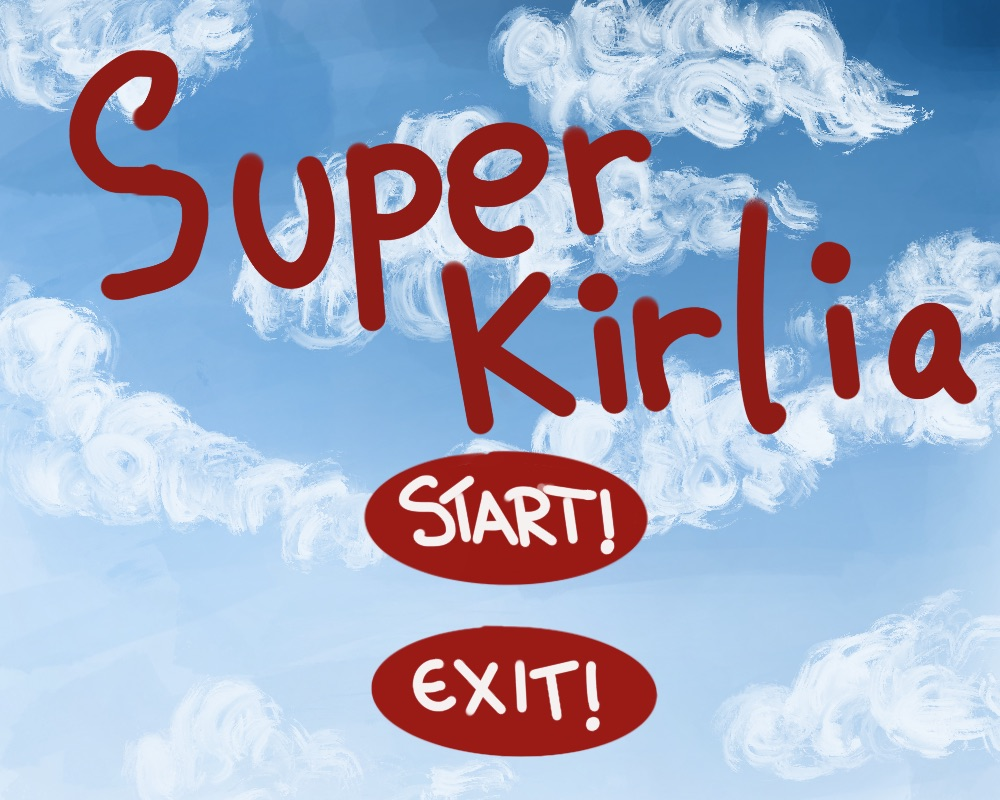
\includegraphics[scale = 0.37]{menu}

\newpage

\section{Dokumentacija rada - Kako je teklo rađenje projekta}
Projekt sam odlučila raditi sama, te je tako na meni bio zadatak da smislim kako će igra izgledati i kako će funkcionirati. Budući da Processing nema neku klasu kao što je Button u Javi, tako sam najprije odlučila napraviti tu klasu radi lakšeg baratanja s gumbima. Isto tako, radi lakšeg snalaženja u kodu i radi lakšeg baratanja s interakcijama između aktera unutar igre, napravila sam klase koje označavaju upravo novčiće koje se trebaju skupljati, klasu koja označava Kirliu (tj glavnog lika), klasu koja označava neprijatelja, klasu koja označava platforme na koje se može skakati i ostalo. Isto tako, postoji jedna posebna klasa koja predstavlja level, i ona se brine da se sve crta na svojem mjestu, provjerava pomoću raznih funkcija da li je novčić skupljen, da li je neprijatelj dotaknut; bavi se kretanjem samog lika.
Jedan od izazova je bilo skakanje samog lika, i hodanje po površinama. (NAPOMENA: Moja greška je što prije pisanja samog koda nisam malo više istražila o postojećim bibliotekama. Naime, postoji biblioteka Box2d koja bi mi puno olakšala kretanje po površinama. Moje rješenje nije koristilo tu biblioteku). Nakon što sam sve to napravila, na red je došlo samo crtanje svega. Program koji sam koristila naziva se Procreate, (link: \url{https://procreate.art/}). To je program koji je napravljen za tablete, a kako ja imam iPad, mogla sam ga koristiti. Program inače nije besplatan, ali nije ni skup. Cijena programa je 9.99 američkih dolara. (Program se može kupiti odjednom, nema mjesečnih preplata!). Nacrtala sam pozadinu, početni zaslon, dva završna zaslona, levele, glavnog lika, novčić i neprijatelja. Glavni lik je jedino što nisam sama smislila, već je to samo precrtana slika pokemona pod nazivom Kirlia. Budući da Procreate ima mogućnost snimanja zaslona, postoje i snimke mog crtanja tih stvari. Snimke su priložene unutar foldera zajedno sa ovim seminarom. Sam rad je trajao više dana. Najviše vremena sam izgubila na probavanje raznih mehanika za kretanje, skakanje, popravljanje samog skakanja i crtanje.
\newpage

\section{Dokumentacija, opis funkcija i klasa}
Kao što sam već rekla, cijeli kod je komentiran, pa u ovom poglavlju neću pretjerano objašnjavati posebno svaku funkciju ili klasu, već su općenito reći što svaka klasa označava.
Klase su sljedeće: Button, ButtonMenu, ButtonExit, Character, Coin, Enemy, Kirlia, Level, Point, Rectangle.

Također je opisan skup funkcija u datoteci InputControl, koje opisuju odgovor programa na unos (pritisak/otpuštanje tipke) sa tipkovnice/miša.

\subsection{Button}
Klasa koja predstavlja gumb. Klasa je abstraktna, što znači da se u glavnom programu treba napraviti konkretan razred koji govori što će taj gumb raditi. Naravno, da bi gumb radio, treba imati funkcije koje govore što se događa kad se klikne mišem, a u glavnom programu u funkciji mousePressed() se treba pozvati ista ta funkcija, ali od gumba.
\subsection{ButtonMenu}
Klasa koja nasljeđuje klasu Button, predstavlja gumb na koji - kada kliknemo - pokreće igru.
\subsection{ButtonExit}
Klasa koja nasljeđuje klasu Button, predstavlja gumb na koji - kada kliknemo - omogućuje izlazak iz igre. 
\subsection{Character}
Klasa predstavlja lika prostoru. Taj lik ima koordinate, tj položaj na kojem se nalazi, visinu, širinu, i može se kretati. Klase Kirlia i Enemy nasljeđuju upravo ovu klasu.
\subsection{Kirlia}
Klasa koja predstavlja lika, glavnog lika kojeg igrač upravlja. Zato ta klasa ima funkcije koje se bave kretanjem, skakanjem, i pritiskanjem strelica, ili slova 'ASWD'.
\subsection{Enemy}
Klasa koja predstavlja neprijatelja, te se objekti te klase same pokreću. Poslije konstrukcije jednog takvog objekta, može se točno definirati koliko je taj lik širok, visok, koliko se daleko može kretati, kako će izgledati i ostalo.
\subsection{Coin}
Klasa predstavlja novčić kojeg Kirlia mora skupiti. Ovo je relativno jednostavno klasa.
\subsection{Point}
Klasa predstavlja točku, ili točnije vektor od 2 dimenzije.
\subsection{Rectangle}
Klasa predstavlja platformu po kojoj Kirlia može hodati. Ime je možda nezgodno, ali to ime je dano jer platforme nalikuju na pravokutnike. 
\subsection{Level}
Ovo je klasa koja ima najviše funkcija, i klasa koja ima najbitnije funkcije. Klasa se brine da cijela igra funkcionira kako spada. Ova klasa omogućava kretanje lika, skakanje lika, skupljanje novčića i ostalo.
\subsection{InputControl}
Ovo je skup funkcija koje opisuju respons programa na:
\begin{itemize}
\item Pritisak tipki na tipkovnici koje u igrama klasično opisuju kretanje
\item Otpuštanje tipki na tipkovnici koje u igrama klasično opisuju kretanje
\item Klik na mišu
\end{itemize}
\newpage

\section{Moguća poboljšanja}
\begin{itemize}
  \item Dodavanje dodatnog menija koji potvrđuje da želimo izaći iz igre (npr. pita korisnika "Are you sure you want to exit?" sa opcijama "Cancel" i "Yes, exit!")
  \item Dodavanje barem još jednog levela
  \item Dodavanje nove pozadine i mogućnost mjenjanja pozadine
  \item Korištenje Box2d biblioteke 
  \item Dodavanje još nekoliko različitih vrsta neprijatelja
  \item Dodavanje mogućnosti skupljanja novčića različitih vrijednosti
  \item Dodavanje mogućnost borbe protiv neprijatelja
  \item Dodavanje gumba koji vraća igrača iz levela na početni zaslon
  \item Dodavanje multiplayera
  \item Prikazivanje broja bodova i života na kraju igre
  \item ...
\end{itemize}
\newpage

\section{Literatura}
\begin{itemize}
  \item \url{https://processing.org/reference/}
  \item \url{https://www.youtube.com/watch?v=DLryAXsIZ04}
\end{itemize}

\newpage


\clearpage

\hfill

\end{document}
